\documentclass[10pt,journal,compsoc]{IEEEtran}
\usepackage{subfiles}
\usepackage{url}
\usepackage[pdftex]{graphicx}
\usepackage{amsmath}
\usepackage{xspace}
\usepackage{multirow}
\usepackage{amssymb}
\usepackage{algorithm}
\usepackage{subfig}
\usepackage[noend]{algpseudocode}
\renewcommand{\algorithmicrequire}{\textbf{Input:~}}
\renewcommand{\algorithmicensure}{\textbf{Output:~}}
\newcommand\ovr[1]{\overrightarrow{#1}}
\newcommand\myeq{\mkern1.5mu{=}\mkern1.5mu}
\usepackage{booktabs}
\usepackage{array}
\usepackage{color}
\usepackage{listings}
\usepackage{placeins}
\usepackage{enumitem}
%%%%%%
% Notes: 
% plot grouping/hue +
% table smallcaps +
% Time score memory center +
% Abstract
% Differences between infuser and us+
% time skecth diff between us +
% neden 0.005 +
% active vertex colors +

% GRID PARAM SEARCH
% Performance comparison vs others (why slowed down?)
% Error-Adaptive rebuilding sat
%%%%%
\ifCLASSOPTIONcompsoc
  \usepackage[nocompress]{cite}
\else
  \usepackage{cite}
\fi

\ifCLASSINFOpdf
\else
\fi
\newcommand\ggx[1]{\textcolor{blue}{#1}}

\newcommand\MYhyperrefoptions{bookmarks=true,bookmarksnumbered=true,
pdfpagemode={UseOutlines},plainpages=false,pdfpagelabels=true,
colorlinks=true,linkcolor={black},citecolor={black},urlcolor={black},
pdftitle={Bare Demo of IEEEtran.cls for Computer Society Journals},%<!CHANGE!
pdfsubject={Typesetting},%<!CHANGE!
pdfauthor={Gokhan Gokturk, Kamer Kaya},%<!CHANGE!
pdfkeywords={Influence Maximization, Graph Processing, Graph Sampling, Fused Sampling, Memory Access Regularization, Count-Distinct Sketch}}%<^!CHANGE!

\newcommand\acro{{\sc{HyperFuseR\xspace}\xspace}\xspace}
\usepackage{xcolor}
\newcommand\kktodo[1]{\textcolor{red}{#1}}



\newcommand\minspeedup{{{3.5\xspace}\xspace}\xspace}
\newcommand\maxspeedup{{{11\xspace}\xspace}\xspace}

\newcommand\maxspeedupTIM{{{1500\xspace}\xspace}\xspace}
\newcommand\maxspeedupIMM{{{27.87\xspace}\xspace}\xspace}
\newcommand\maxspeedupSKIM{{{11\xspace}\xspace}\xspace}

\begin{document}

\title{Fast and Error-Adaptive Count-Distinct Sketch
\\for Influence Maximization}


\author{G\"{o}khan~G\"{o}kt\"{u}rk
        and~Kamer~Kaya% <-this % stops a space
\IEEEcompsocitemizethanks{\IEEEcompsocthanksitem G. G\"{o}kt\"{u}rk and K. Kaya are with Computer Science and Engineering, Faculty of Engineering and Natural Sciences, Sabanci University, TR~34956, Istanbul, Turkey.}% <-this % stops a space
%\thanks{Manuscript received April 19, 2005; revised August 26, 2015.}}
}
%FIXME



% \markboth{Journal of \LaTeX\ Class Files,~Vol.~14, No.~8, August~2015}%
% {Shell \MakeLowercase{\textit{et al.}}: Bare Advanced Demo of IEEEtran.cls for IEEE Computer Society Journals}


\IEEEtitleabstractindextext{%
\begin{abstract}
Influence maximization~(IM) is the problem of finding a seed vertex set that maximizes the expected number of vertices influenced under a given diffusion model. Due to the NP-Hardness of finding an optimal seed set, approximation methods are frequently used for IM. In addition to high-quality yet expensive approximation algorithms, to meet with the scale of today's networks, lightweight, sketch-based approaches, which do not simulate the process exactly, have been proposed in the literature. As expected, the quality of the seed sets for the latter is inferior to those of the former. In this work, we describe a fast, error-adaptive approach that leverages Count-Distinct sketches and the recently proposed hash-based, fused sampling. To estimate the vertex set sizes influenced throughout the simulations, we use per-vertex Flajolet-Martin sketches where each sketch register corresponds to a sample sub-graph. During the diffusion simulations, the reach set cardinalities of a single vertex are stored in adjacent registers in memory. This allows the proposed algorithm to find the number of influenced vertices in a single simulation step in different simulations at once. In addition, thanks to its efficiency and scalability of our parallel implementation can rebuild the sketches after observing large estimation errors. Our experimental results show that the proposed method finds high-quality seed sets  while being up-to $1.7\times$--$27.9\times$ faster on average than a state-of-the-art approximation algorithm. In addition, it is shown to be $3.5\times$--$11.1\times$ faster than a sketch-based approach while producing seed sets with $3\%$--$12\%$ better influence scores.
\end{abstract}
% Note that keywords are not normally used for peer review papers.
}


\maketitle

\IEEEdisplaynontitleabstractindextext
\IEEEpeerreviewmaketitle


\ifCLASSOPTIONcompsoc
\IEEEraisesectionheading{\section{Introduction}\label{sec:introduction}}
\else
\section{Introduction}
\label{sec:introduction}
\fi

The study of efficient information/influence propagation in networks becomes an important area of research with several applications from many fields, such as viral marketing~\cite{leskovec2007dynamics, trusov2009effects}, social media analysis~\cite{zeng2010social, moreno2004dynamics}, and recommendation systems~\cite{lu2012recommender}.
As the study of these networks is imperative for educational, political, economic, and social purposes, a high-quality seed set to initiate the diffusion may have critical importance.
Furthermore, since the diffusion analysis may be time-critical, or increasing its coverage may be expensive in terms of computing resources and time, novel and efficient approaches to find good vertex sets that propagates the information/influence effectively is essential.

Influence maximization is the problem of finding a subset $S \subset V$ of $K$ vertices in a graph $G = (V, E)$ with the vertex set $V$ and edge set $E$ such that $S$ reaches the maximum reachability under some diffusion model $M$. In addition to introducing the problem, Kempe et al.~\cite{kempe2003maximizing} proved it to be NP-hard and provided a greedy Monte-Carlo approach that has a constant approximation for the optimal solution. This greedy approach is one of the most frequently applied algorithms for IM. The time complexity of the greedy algorithm, estimating the $\sigma$ influence score, running $R$ simulations, and selecting $K$ seed vertices is $\mathcal{O}(KRn\sigma)$ for a graph with $n$ vertices. Although they perform well in terms of seed-set quality, in consequence, the greedy Monte-Carlo solutions are impractical for real-life networks featuring millions of vertices. Due to this reason, many heuristics and proxy methods have been proposed in the literature~\cite{MixGreedy, narayanam2010shapley, kimura2007extracting, chen2010PMIA,chen2010LDAG, kim2013scalable, cohen2014sketch, goyal2011simpath, jung2012irie,cheng2014imrank,liu2014influence,galhotra2016holistic}.

%%%%%%%%%%%%%%%%%%%%%%%%%%%%%%%%%%%%%%%%%%%%%%%%%%%%%%
%%%%%%%%%%%%%%%%%%%%%%%%%%%%%%%%%%%%%%%%%%%%%%%%%%%%%%
 
% However, these simulation-based, greedy algorithms provide the best possible approximation guarantees. Therefore they are considered as the gold standard for IM.  

Simulating a greedy algorithm in parallel is an obvious and straightforward workaround to reduce the execution time of IM kernels and make them scalable for large-scale networks. However, for large networks, a greedy approach with a good approximation guarantee does not come cheap even if a large number of processing units/cores are available on networks with billions of vertices and edges. Following similar attempts in the literature, we propose a parallel, sketch-based greedy approach that approximates the Monte-Carlo processes. The proposed approach does not exactly count the number of influenced vertices. Instead, it leverages Count-Distinct sketches. 
in this work, we apply parallelism in multiple levels; thread-level and instruction-level parallelism. While modern compilers employ instruction-level parallelism effectively and automatically for applications with regular memory access patterns, graph kernels are usually harder to deal with. The irregularity of the neighbor IDs. ..... due to their irregular memory access patterns, it is not a straightforward task for graph processing kernels.  Besides, vectorization attempts on such kernels typically fail to provide substantial speed-up in performance. 

In this work;
\begin{itemize}[leftmargin=*]
\item We propose, \acro\footnote{\url{https://github.com/ggokturk/infuser}}, an open-source, a blazing-fast, and accurate Influence Maximization algorithm. The proposed scheme samples the edges as they are traversed across several simulations. Thus, sampling, diffusion, and count-distinct processes are fused for all simulations. 

\item Running concurrent simulations on per-vertex count-distinct sketches reduces the number of memory accesses. While traversing an edge, any number of diffusion simulations can be performed between vertices, using only a single integer (8-bit) per vertex for each simulation. 

That is when the simulations traverse the same edge within close time intervals, the edge is accessed only once as long as the simulation timelines allow \acro to do so. The suggested approach, therefore, decreases the pressure on the memory management unit. In relation, for the cascade model, we employ a vector compute unit, near maximum efficiency to regularize memory accesses. 
%\item In addition to instruction-level parallelism, we parallelize \acro on multi-core architectures.

\item \acro{} can process very large graphs with millions of vertices and hundreds of millions of edges under a minute, without compromising the quality of results. For large graphs, due to its race condition indifferent nature, performance scales near linearly with the number of threads available. While processing the graph, only we few GBs of memory is used, mostly for storing the graph itself. 

% \item \acro can be around $200000\times$ faster compared to the traditional greedy approaches. It is usable on large graphs that have been considered as {\em too large} in the literature. For instance, the new algorithm runs in $2.09$, $0.08$, $0.36$ seconds on networks {\tt Amazon}, {\tt NetHEP}, {\tt NetPhy} with 16 threads where the sequential baseline takes $141.3$, $259.1$ and $1725.2$ seconds, respectively. In fact, with a 302,400 seconds~(3.5 days) timeout, the sequential baseline can process only the above-mentioned 3 (out of 12) real-life graphs, having 1.2M, 58.9K and 231.5K edges. On the other graphs, the original algorithm cannot complete the simulations within the time limit. However, \acro{} completes all of 12 graphs around 1200 seconds in total, where the maximum is 654 seconds for the {\tt Orkut} network having 3.1M vertices and 117.2M edges. 

\item We evaluate the performance, memory consumption, and influence score with a state-of-the-art influence maximization algorithms {\sc Skim}~\cite{cohen2014sketch}, {\sc Tim+}~\cite{tim}, {\sc Imm}~\cite{minutoli2019fast} in order to accurately position the performance of \acro{} in the IM literature. The experiments show that \acro is $\minspeedup\times$—$\maxspeedup\times$ faster than state-of-the-art while still being better in comparison in terms of scores, and using a comparable amount of memory.

\end{itemize}

The paper is organized as follows: 
In Section~\ref{sec:background}, we present 
the background on IM and introduce the mathematical notation. 
Section~\ref{sec:method} describes the proposed approach in detail.
In Section~\ref{sec:evaluation}, a thorough performance comparison over the traditional algorithms is provided by conducting experiments on various real-world datasets and influence settings. Besides, a comparison with the state-of-the-art from the literature is given.
Section~\ref{sec:relatedwork} presents a comparative overview of the existing work. Finally, Section~\ref{sec:conclusion} discusses future work and concludes the paper.






%%%%%%%%%%%%%%%%%%%%%%%%%%%%%%%%%%%%%%%%%%%%%%%%%%%%%%
%%%%%%%%%%%%%%%%%%%%%%%%%%%%%%%%%%%%%%%%%%%%%%%%%%%%%%
\section{Notation and Background}\label{sec:background}

Let $G = (V,E)$ be a directed graph where the $n$ vertices in $V$ represent the agents, and $m$ edges in $E$ represent the relations between the agents in $V$.
The neighborhood of a vertex $u \in V$ is denoted as $\Gamma_{G}(v) = \{v: (u,v) \in E\}$. 
A graph $G' = (V',E')$ is a sub-graph of $G$ if $V' \subseteq V$ and $E' \subseteq E$. 
Diffusion probability on edge $(u, v) \in G$ is noted as $w_{u,v}$.
$w_{u,v}$ can be determined either by the diffusion model or according to the strength of $u$ and $v$'s relationship in the data.

\begin{table}[!ht]
    \caption{Table of notations}
    \label{tab:notation}
    \centering
    \begin{tabular}{|l|p{0.7\linewidth}|}
        \hline
        Variable & Definition  \\
        \hline
        $G = (V,E)$     & Graph $G$ with vertices $V$ and edges $E$ \\
        $\Gamma_G(v)$   & Neighborhood of incoming edges to vertex $v$ in graph $G$\\ %%FIXME
        $w_{u,v}$       & Probability of $u$ directly influencing $v$ \\
        %$SCC(v) $       & Strongly connected component of vertex $v$\\
        $R_{G}(v)$      & Reachability set of vertex $v$ on graph $G$\\
%        $\overline{R_{G}(v)} & Complement of the vertex set $R_{G}(v)$\\
        \hline\hline
        $S$             & Seed set to maximize influence\\
        $K$             & Size of the seed set\\
        $\mathcal{R}$   & Number of Monte-Carlo simulations performed\\
        $\sigma_{G}(S)$ & Influence score of $S$ in $G$, i.e., expected number of vertices reached from $S$ in $G$\\
        % $\sigma_{G}{(S,v)}$          & Marginal influence gain by adding vertex $v$ to seed set $S$\\
\hline\hline
        %$p$             & Sampling probability for edges\\
%        $P(s,v)_r $     & Random probability generated for selecting edge vertices $s$ to $v$ in simulation $r$\\
        $X_{r..n}$      & Slice of Vector X between r and r+n(not including)\\
        $h(u,v)$        & Hash function for edge $\{u,v\}$\\
        $h_{max}$       & Maximum value hash function $h$ can return\\
        %$X_r$           & Random number/hash generated for simulation $r$  \\
        \hline\hline
        $B$             & Batch size\\
        $e$             & Estimated reachability set size\\
        % $[a, \ldots, a]_B$      & Vector of size $B$, contains all $a$\\
        $M_u[j]$        & $j$th sketch register for vertex $u$\\
        $\varsigma $    & Influence gained before last sketch build\\
        $\sigma $       & Influence Score\\
        $\delta$        & Marginal Gain after last sketch build\\
        $\epsilon_{global}$    & Global estimation error threshold\\
        $\epsilon_{local}$    & Local estimation error threshold\\ 
        $\epsilon_{conv}$    & Non-convergenced vertex threshold\\
      %  $x[[i, j]]$   & Slice of vector  $x$ between indices $i$ and $j$, not including $j$ \\ 
        \hline         
    \end{tabular}
\end{table}
\subsection{Influence Maximization}

Influence Maximization aims to find a seed set $S \subseteq V$ among all possible size $K$ subsets of $V$ that maximizes an {\em influence spread function} $\sigma$  when the diffusion process is initiated from $S$. Although we focus on undirected graphs, for IM, the graph can be directed or undirected depending on the initial construction. Figure~\ref{fig:xx} shows a~(Fig.~\ref{fig:ic}) and directed~(Fig.~\ref{fig:wc})
graph for which the weights on the edges are diffusion/influence probabilities. 

\begin{figure}[!ht] 
    \centering
  \subfloat[\small{IC}\label{fig:ic}]{%
       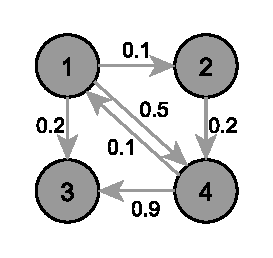
\includegraphics[width=0.50\linewidth]{images/ic.pdf}}
  \subfloat[\small{WC}\label{fig:wc}]{%
        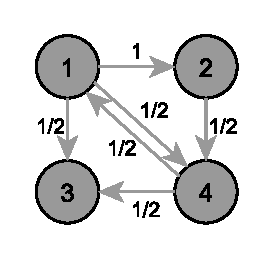
\includegraphics[width=0.50\linewidth]{images/wc.pdf}}
    \\% IMAGES HERE
  \caption{\protect\subref{fig:ic} 
The directed graph $G = (V, E)$ for Independent Cascade with independent diffusion probabilities. 
\protect\subref{fig:wc}
The directed graph was obtained from the directed one by setting the diffusion probabilities of incoming edges to $1 / |\Gamma_G(v)|$ for each vertex $v \in V$. 
  }
  %\label{fig_ic_model} 
  \label{fig:xx} 
\end{figure}

The $\sigma_{G, M}(\cdot)$ influence spread function calculates the {\em estimated} number of agents / nodes / vertices affected~(activated) through a $M$ diffusion model. 
We eliminate $M$ from the notation for the sake of elegant simplicity; in the remainder of the text, $\sigma_{G}$ refers to $\sigma_{G, M}$.
In the literature, {\em independent} and {\em weighted cascade}~(IC and WC), and 
{\em linear threshold}~(LT)~\cite{kempe2003maximizing} are some of the widely recognized diffusion models for IM. 

\begin{itemize}[leftmargin=*]
\item The {\bf Independent Cascade} process performs in iterations and activates the $v$ vertex if one of its (incoming) edges, $(u, v)$, is 
used during the iteration of diffusion, which has an expected probability of $w_{u, v}$, because $u$ was already influenced in the previous rounds. 
Activation probabilities are independent (from each other and previous activations) in the {\em independent} variant which we concentrate on in this paper, as in Figure~\ref{fig:ic}.
In theory, there can exist parallel and  independent $\{u, v\}$ edges in $E$. In practice, they are merged to a single $\{u,v\}$ edge via preprocessing. 

\item The {\bf Weighted Cascade}  model is a variant of the independent cascade that uses the structural properties of vertices to set weights as shown in Figure~\ref{fig:wc}.
The method, as described in ~\cite{MixGreedy}, sets $w_{u, v} = 1 / d_v$ where $d_v$ is the number 
of incoming edges of $v$ for introducing weight values(which in the original graph is equal to $\Gamma G(v)$).
Therefore, if $v$ is triggered after the last round with $\ell$ neighbors, its activation probability in the new round is $1-( 1-1 / d_v)^\ell$. 

%$ {|E^G_{u,v}|}/{|E^G_{u}|}$ where $|E^G_{u,v}|$ is the number of parallel $\{u, v\}$ edges and $|E^G_{u}|$ is the number of $\{u, .\}$ edges, i.e., all of $u$'s edges in the undirected graph.

\item{\bf Linear threshold} generalizes the cascade models and activates the $v$ vertex once the cumulative activation coming from the neighbors of $v$ exceeds the $\theta v$ threshold. 
All the $\{u, v\}$~(or $(u, v)$ in the directed graph) edges 
with active $u$ vertices are taken into account in the process. Vertex $v$ is activated~\cite{kempe2003maximizing} when the number of these edge weights reaches $\theta v$.  
Therefore, the cascade models are special variants of the linear threshold model with $\theta v = 0 $. 

%Each edge $e=(s,v) \in E$ has a weight $w_{s,v}$. Each vertex $v$ has incoming edge list $Adj^{-1}(v)$ and $\sum_{s\in Adj^{-1}(v) }{w_{s,v}} \leq 1$. Also, each vertex $v$ has associated with a threshold $\theta_v$. Initially, $\theta$ is sampled uniformly, and seed set is set as activated. Then, until convergence is reached simulation ran to transfer $w_ij$ values from activated vertices to their neighborhoods, activating each vertex $v$ that reach $\theta_v$ value. Weights can be uniform i.e 0.1, 0.01, or 0.001 for all edges, as we observed in many work. 

\item {\bf Triggering} proposed by Kempe et al.\cite{kempe2003maximizing} to generalize of previous models mentioned above. In the triggering model, each neighbor has a probability to influence vertex $v$. The diffusion process chooses a random subset of vertices called the "triggering set" to activate vertices at each instance.
\end{itemize}

The complexity analysis stays consistent for many diffusion models including {\em Independent Cascade}~(IC), {\em Linear Threshold}~(LT),  models. 
% Current studies focus on reducing the number of simulations run \cite{goyal2011celf++, goyal2011simpath}, sketch-based speedup methods\cite{SKIM}, and proxy methods that solve similar yet simpler problems \cite{kempe2003maximizing}. %FIXME too many methods, one french paper in python
%\cite{kempe2003maximizing} 
We concentrate on the independent cascade model in this paper, but the proposed methods are also relevant to the other models in the literature.
%  \[ \sigma(S^*)=\argmax_{S\subseteq V \land |S| \leq k } \sigma_{G}(S) \]

%is a simple diffusion model that Vertex v can be activated by any of incoming edges from activated vertices w with probability $p$. Given a seed set $S$ and influence probability $p$, the cascade model starts from the activated seed set and tries to diffuse until each of the out-going edges of active vertices are considered. The diffusion process considers all edges only once.

\subsection{Count-Distinct Sketch}\label{sec:sketch}
The count-distinct problem is the problem of finding the number of distinct elements in a stream with non-distinct elements. Computing reachability sets of a vertex is a similar problem; the cardinality of all vertices visited is calculated while traversing sample sub-graphs from the given vertex. Exact cardinality calculations require memory proportional to the cardinality. 

The reachability set of a vertex is a distinct union of all connected vertices' reachability sets. Many other Influence Maximization methods exploit this property to some degree. 

The methods based on Reverse reachability and Bottom-Up Traversal utilizes this property directly to merge reachability sets of connected vertices to estimate vertices influence.
MixGreedy method goes one step further; it utilizes that all vertices in a connected component that have the same reachability set in undirected graphs. So, for a sample graph, all reachability sets can be found in a single graph traversal. 

For directed graphs, storing reachability sets for all vertices and merging these sets are infeasible for non-trivial graphs. 
If one-hot vectors are used to store reachability sets for constant insertion time, $O(n^2\mathcal{R})$ bits of memory is required and each merge operation has $O(n)$ time complexity. 
if Disjoints sets are used for storing reachability sets; $(n\bar{\sigma}\mathcal{R})$ memory is required to store all reachability sets, and each merge operation has $O(ackermann'(\sigma))$ complexity.

Count-distinct sketches have nice properties for such problems; Flajolet–Martin algorithm\cite{flajolet1985probabilistic} can estimate the cardinality of distinct elements in reachability sets with a constant number of registers($J$), and most importantly union of these sets can be done in a constant number of operations.


Flajolet–Martin algorithm only stores how rare elements are in a multi-set.The rarity of the elements is often computed by counting leading zeros in the item's hash values.  The registers are initialized with zero values in beginning. Items are added by storing the longest leading zero count. Cardinality estimation can be done by taking 2 to the power of the stored value. Multiple registers and hash functions, $M[j]$ and $h_j$, are commonly used to reduce variance.
Adding item $x$ to sketch $M$, and its result $M'$ is shown in equation~\ref{eq:sketch-add}.

\begin{equation}
    \label{eq:sketch-add}
    M'[j] = max(M[j],clz(h_j(x)) ~ \forall j\in(0,J]
\end{equation} where $clz$ is count leading zeros function and $J$ is the number of sketch registers.

The merge operation for two sketches, $M_u$,$M_v$, can be performed by computing the pairwise maximum of the registers. Formally; 
\begin{equation}
    \label{eq:sketch-merge}
    M'[j] = max(M_u[j],M_v[j]) ~ \forall j\in(0,J]
\end{equation} 
where $M'$ is union of set and $J$ is number of sketch registers.

Average of longest running zeros can be used compute the cardinality and the result is divided to correction factor $\phi \approx 0.77351$ to correct hash collisions.
\begin{equation}
    \label{eq:sketch-estimate}
    e = 2^{\bar{M}}/\phi
\end{equation} 
where $e$ distinct cardinality and $\bar{M}$ is the mean of the registers.

In this work, we utilize a variant of Flajolet–Martin sketch; since multiple Monte-Carlo simulations are performed to calculate estimated influence, we use one register per simulation, and take the average of longest leading zero counts to calculate the average cardinality of reachability sets. Merge operations are performed if and only if there is an edge between the respective simulation. 

\section{Method}\label{sec:method}

\subsection{Hash-based Fused Sampling}
The probabilistic nature of cascade models requires sampling sub-graphs $\hat{G}$ from $G = (V, E)$ to simulate the diffusion process.  Sampling can be a dominating factor in processing; sampling may demand multiple passes on the graph, if samples are memoized, multiple times of the graph size needs to be stored.
In this work, we borrow hash-based fused sampling from {\sc InFuseR}\cite{infuser}. By using a hash-based fused sampling, we eliminate the necessity of in-memory creation and storage of the sample sub-graphs.
While processing an edge, it is considered for all possible samples.
It is sampled or skipped depending on the outcome of the hash-based random value. The hash function used is given in equation \ref{eq:hash}.
\begin{equation}
    \label{eq:hash}
    h(u,v) = \mbox{{\sc Murmur3}}(u||v)~mod~2^{31}  
\end{equation}
where $||$ is the concatenation operator. 

We have tried a few other hash algorithms as well; Ideally, we chose {{\sc Murmur3}} due to its simplicity and good avalanche behavior with maximum bias $0.5 \% $\cite{MurmurHash3Performance}.

For performance considerations, edge hash values were pre-computed in our work and only existing pairs were considered. The trade-off between extra memory and computation here maybe not be applicable for different computation architectures and faster/simpler hash functions.

Although the above-mentioned approach generates a unique hash value for each edge, and hence a unique sampling probability, different simulations require different probabilities.

\begin{figure}[!ht] 
    \centering
    %\subfloat[\label{fig:toy}]{%
    %   \includegraphics[width=0.47\linewidth]{sims-a%}}%  \\
    \subfloat[\label{fig:sims}]{%
        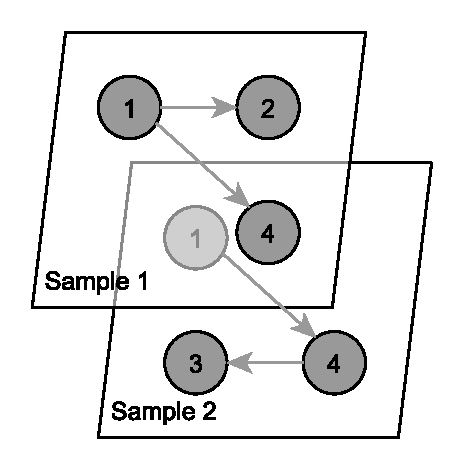
\includegraphics[width=0.5\linewidth]{images/samples.pdf}
    } 
    \subfloat[\label{fig:fused}]{%
     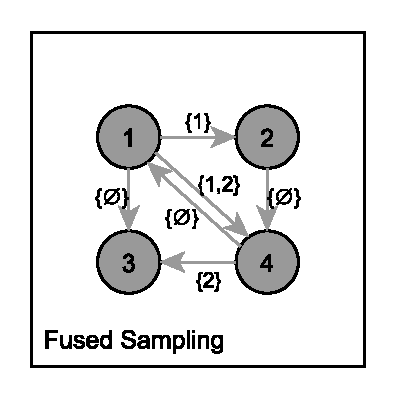
\includegraphics[width=0.5\linewidth]{images/fused.pdf}}
  \caption{
  %\protect\subref{fig:toy} The toy graph 
  \protect\subref{fig:sims} Two sampled subgraphs of the toy graph from Figure~\ref{fig:ic} with 4 vertices and 6 edges.
  \protect\subref{fig:fused} The simulations are performed in a way to be fused with sampling. Each edge is labeled with the corresponding sample/simulation IDs. 
  }
  \label{fig:traversal} 
\end{figure}


Multiple deterministic random values for each edge is generated by using the edge hash values and random numbers $X_r$ associated with each simulation $r$. 
Sampling probability of $(u, v)$ for simulation $r$, $P(u, v)_r$, is computed as follows; First, $h(u,v)$ is XOR'ed with a uniformly randomly chosen $X_r \in_R [0, h_{max}]$ and the result is normalized by dividing the value to the upper limit of the hash value $h_{max}$. Formally,
\begin{equation}
    \label{eq:hash_prob}
    P(u,v)_r = \frac{X_r \oplus h(u,v)}{h_{max}}.
\end{equation}

% The edge $\{u,v\}$ is verified to be in the sample if ${\rho}(u,v)_r$ is smaller than or equal to the threshold $w_{u,v}$. 
The edge $\{u,v\}$ is exists in the sample $r$ if and only if  ${P}(u,v)_r$ is smaller than the edge threshold $w_{u,v}$. One of the benefits of this approach is, sampling an edge is only single XOR and compare-greater-than operations. Also, the following control flow branch can be removed using conditional move operations. 
An efficient implementation of this approach will be discussed later in this section.
\begin{figure}[!ht] 
    \centering
    \includegraphics[width=1\linewidth]{./images/CDF.pdf}
    \caption{Cumulative probability function of hash-based sampling probabilities on various real-life networks.}
    \label{fig:prob-cdf} 
\end{figure}
Using a strong hash function such as {{\sc Murmur3}} ensures all bits independently change if the input is changed. This property allows us to generate good enough pseudo-random values for fair sampling. To prove the fairness of random values generated with the hash-based approach, we generated a large number of samples for various real-life networks and graphed the bias of random values $P(u,v)_r$ used while sampling.

% For a given graph $G = (V,E)$, the bias of a sampling probability $x$ is computed as $|(31/2) − E(|H(m)|) / E(|H(m)|))|$ for all $(u,v) \in E$ and $0 \leq r < R$. 
Figure~\ref{fig:prob-bias} shows the bias for 12 real-life networks. The sampling probability distribution with hash-based computation is almost identical to the uniform distribution with small bias.


\begin{figure}[!ht] 
    \centering
    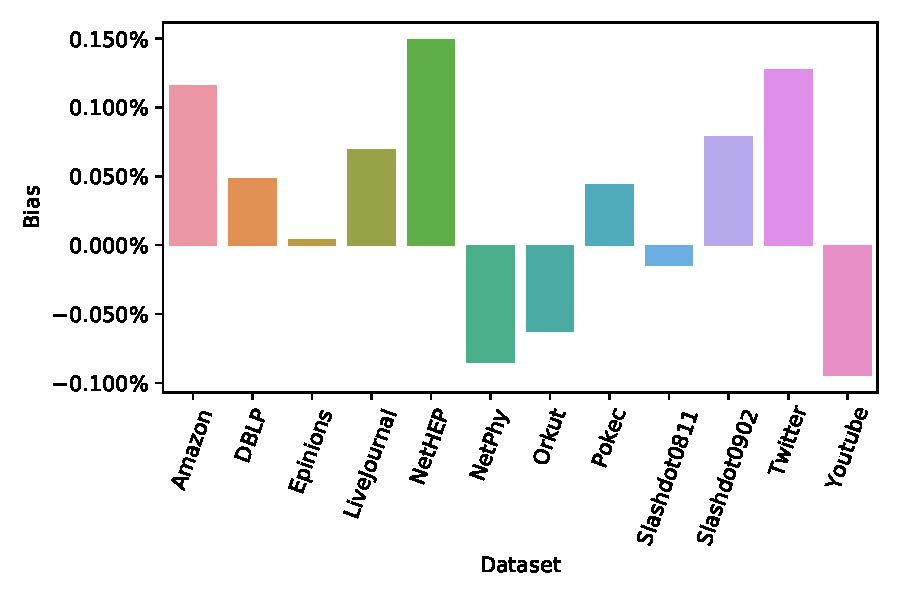
\includegraphics[width=1\linewidth]{./images/bias.pdf}
    \caption{Bias distribution of hash-based sampling probabilities on various real-life networks.}
    \label{fig:prob-bias} 
\end{figure}

%Traditional implementations sample each edge in $G$ once per simulation and store them to construct a sampled subgraph. n
Being able to generate infinitely many samples on-the-fly, allows us to avoid many memory accesses. The only down-side of hash-based fused sampling is that we have to generate all random values,   $P(u,v)_r$, for each edge traversal.  Fortunately, these computations are quite fast on modern computing hardware.

\subsection{Reachability Set Cardinality Estimation}
A greedy solution to the influence maximization problem requires finding a vertex that maximizes marginal influence gain at each step until the seed set size reaches $K$. And, Single vertex influence estimation is the same problem as the count-distinct problem applied to all sample sub-graphs. So, it is possible to use Count-distinct sketches to estimate influence scores in the greedy method. 

We propose an influence maximization method, that utilizes the Count-distinct sketch we mentioned in section \ref{sec:sketch} to estimate averages of distinct elements in sample subgraphs for both time and space efficiency. Algorithm \ref{algo:main} describes the method proposed as follows; 

First, reachability sets of all vertices are initialized with vertices themselves. For all vertices $u$, its $j$th register is set to $M_u[j]=clz(h_j(u))$ meaning $R_{\hat{G}_j}(u) = \{u\}$. Then, we perform diffusion process on the sketch registers. 

Second, the diffusion process is performed between vertex sketches. All vertices added to live vertices set $L$. Then, incoming edges $(u,v)$ for all live vertices are processed. For all simulation $u$ is live, the sketch of both sides are merged and set to $u$ registers. If any of the sketch-registers change, vertex $u$ is added to the next iteration's live vertices set $L'$. After live edges are processed, if the next iteration's live vertices set is smaller than the convergence threshold $\epsilon_c$, the diffusion process concluded. If not, we swap $L$ and $L'$, clear $L'$, and then diffusion processed is repeated. 

In Greedy algorithm\cite{kempe2003maximizing} for each candidate vertex, influence diffusion computations are performed for each vertex.  On the other hand, diffusion on sketch registers allows finding all vertices reachability set. All vertices influence in a single-step distance only computed once. This dynamic programming like property allows fast selection of influence maximizing candidate. Only iterations as much as the diameter of sample graphs are required to converge the sketches. 


After diffusion, the following process is repeated until $K$ vertices are added to the seed set; For all vertex, $u$ reachability set cardinalities, $R_G(S\cup u)$, estimated by merging $mask$ and their sketch registers. The $mask$ used for the sketch of $R_G(S)$ and initialized with zeros. Vertex with maximum cardinality is selected to add to the seed set. Then, the actual Monte-Carlo simulations were performed to compute the reachability set of the seed set. Having actual $R_G(S)$ allows both to calculate estimation errors and to find blocked vertices for all simulations. Blocked vertices skipped in the diffusion step in coming iterations. Besides, the real influence score allows us to know when to rebuild our sketch when the sketches have gone stale.


\begin{figure*}[!ht]
    \begin{center}
    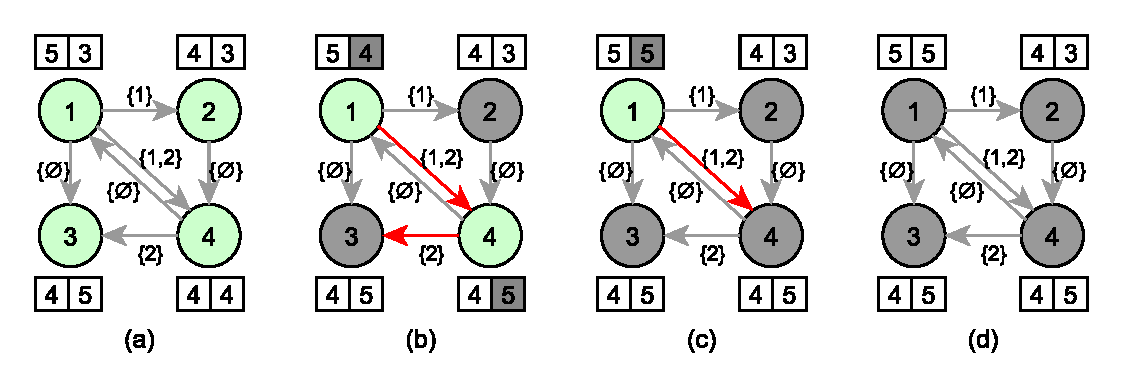
\includegraphics[width=\linewidth]{images/sketch-diffusion.pdf}
    \caption{(a) The initial state on the toy graph for \acro{}; all vertices have set as live(green) and their registers initialized with leading zero count of their hashes. (b) 
    % For all live edges,$e_{ij}$, respective registers are merged and set to source vertex $j$'s register, $M_j \leftarrow Max(M_i, M_j)$. 
    For the live edge between Vertex 1 and 4, the register is set to the maximum of the respective register. Since the first register of vertex 1 is bigger, we only update the second register. Also, the edge between vertex 4 and 3 is only live in simulation 2, so we only set the maximum of those two registers to vertex 4's second register. Notice that, we are moving registers in reverse, from target to source of the edges. We set vertices 1 and 4 as live(green) since their registers have changed in this iteration (c) Vertex 1's register is updated and set as live again since vertex 4's registers are changed.  (d) All vertices have registers converged, there are no live vertices. }\label{fig:hf-processing} 
    \end{center}
    \end{figure*}
\subsection{Error-Adaptive Sketch Rebuilding}

Sketches are very fast approximation methods that often provide less than gold standard results. In our case, sketches are very competent at finding the first few vertices. But, after sketch registers saturate with high values, we observe a significant drop in the quality of results. Register saturation causes the naive count-distinct sketch method to not distinguish between vertices. 

\begin{figure}[!ht]
    \begin{center}
    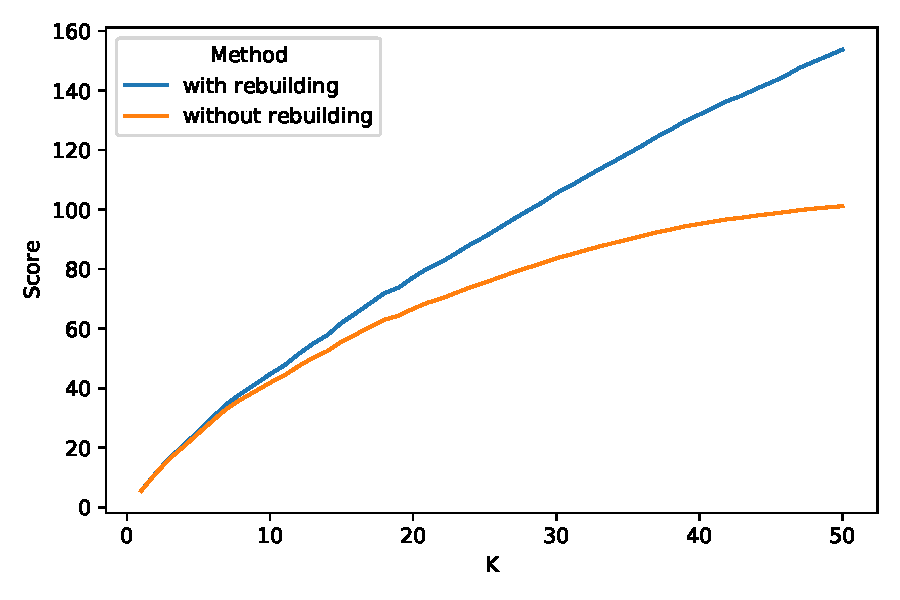
\includegraphics[width=\linewidth]{images/sketch-saturation.pdf}
    \caption{ Effect of register saturation on Amazon dataset using \acro($J=256$) without rebuilding.
     }\label{fig:sketch-saturation} 
    \end{center}
\end{figure}

In figure \ref{fig:sketch-saturation}, we show the effect of register saturation by comparing two methods; one that uses a new sketch, that build on the residual graph after seed sets' reachability is removed, for all iterations. Other, builds the sketch once at the beginning, then only utilizes sketch merge operations to find the seed set. 
Even though at first few vertices expected influence is comparable, we see observe near-linear drop-off in estimated influence.
    

Since building sketches with \acro is very fast, we exploit this by rebuilding sketches after observing large cardinality estimation errors.
After adding vertices to the seed set, \acro performs Monte-Carlo simulations to estimate the reachability of the latent seed set.
The sketches are assumed as stale if the absolute error in estimated total influence score is more than the global threshold, $\epsilon_{global}$, 
and the marginal gain estimation error after the last sketch is larger than a local threshold $\epsilon_{local}$. 

Before rebuilding stale sketches, the reachability set of latent seed set,$R_G(S')$, is marked as visited, 
and considered blocked in their respective simulations while rebuilding the sketches. Then, sketches are rebuild using Monte-Carlo simulations. After rebuilding, $mask$, which holds the cardinality estimate of the seed vertices added after the last rebuild, is cleared with all zeros.

The use of two threshold values allows the algorithm to rebuild after large local errors but skip rebuilding if the error is minuscule relative to the total score. 
If a rebuild is not required, we only update the $mask$ by merging it with the candidate vertex's sketch. 
This approach allows us to keep sketches high quality even after many vertices are added to the seed set, but on the other hand, forces us to perform Monte-Carlo simulations which can be expensive. We reuse the reachability sets of latent seed set, $R_G(S')$, computed by Monte-Carlo simulations. While rebuilding sketches, $R_G(S')$ is used to check whether if a vertex is blocked in a sample.

Other methods mentioned in this paper, doesn't report time spend on calculating the influence scores, 
whereas our method includes the time since it is crucial for keeping sketches in high quality.

\begin{figure*}[!h]
    \begin{center}
        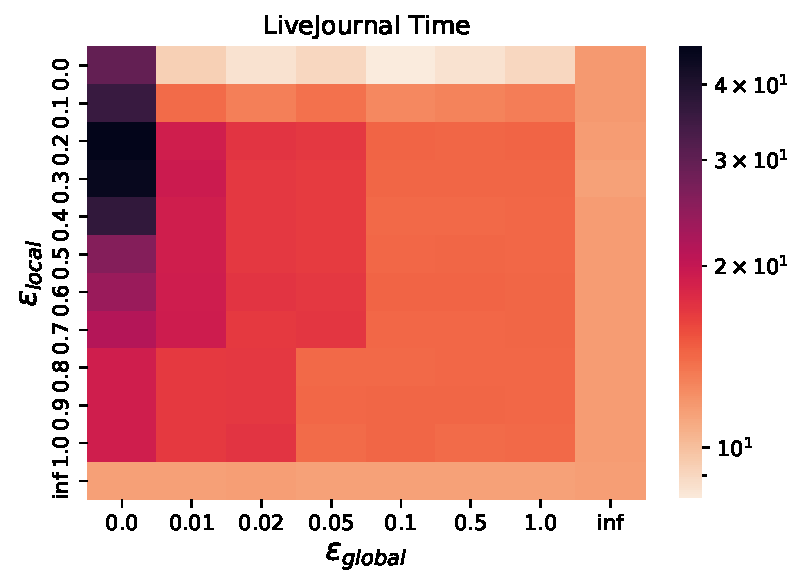
\includegraphics[width=0.33\linewidth]{images/heatmap_LiveJournal_time.pdf}
        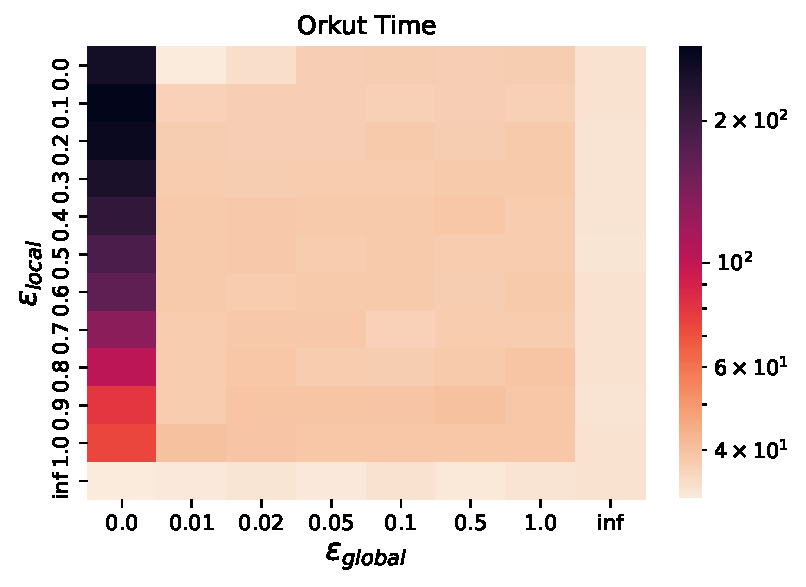
\includegraphics[width=0.33\linewidth]{images/heatmap_Orkut_time.pdf}
        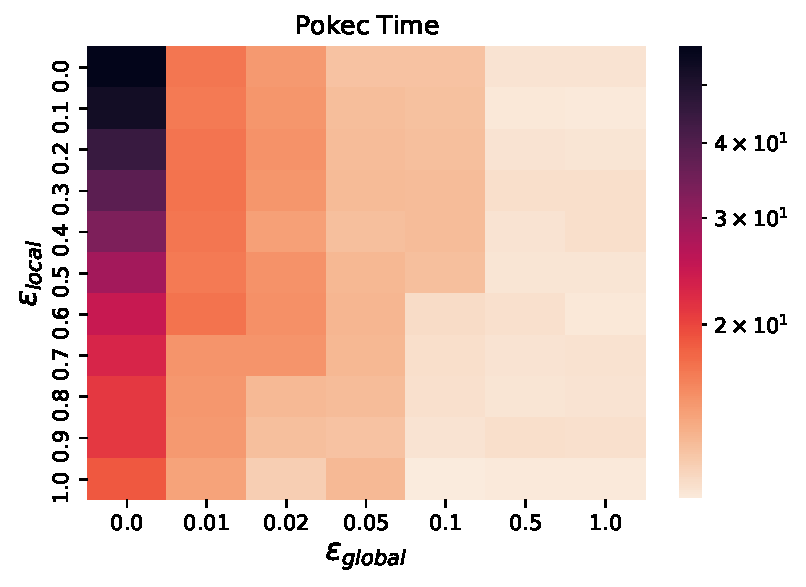
\includegraphics[width=0.33\linewidth]{images/heatmap_Pokec_time.pdf}\\
        
        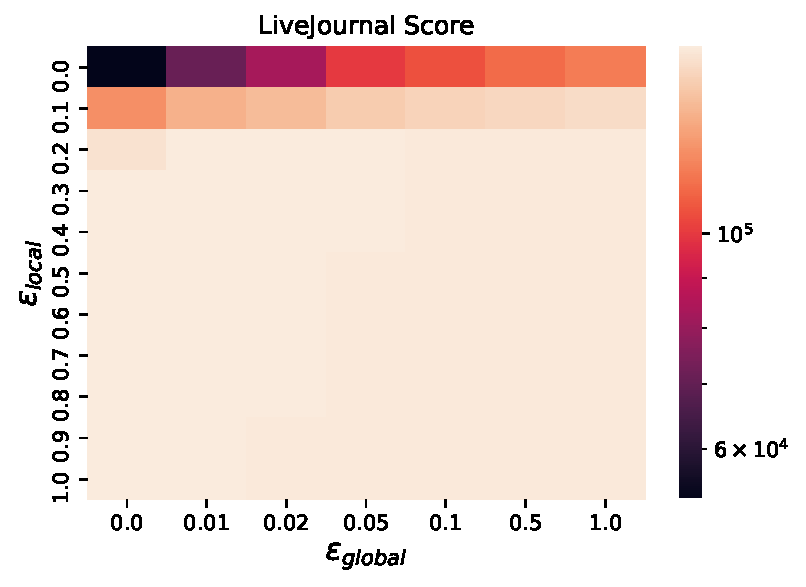
\includegraphics[width=0.33\linewidth]{images/heatmap_LiveJournal_score.pdf}
        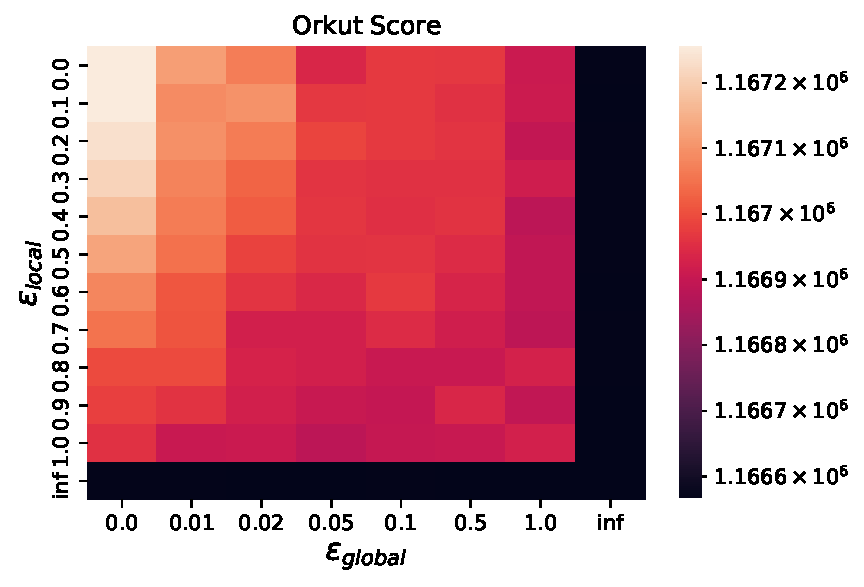
\includegraphics[width=0.33\linewidth]{images/heatmap_Orkut_score.pdf}
        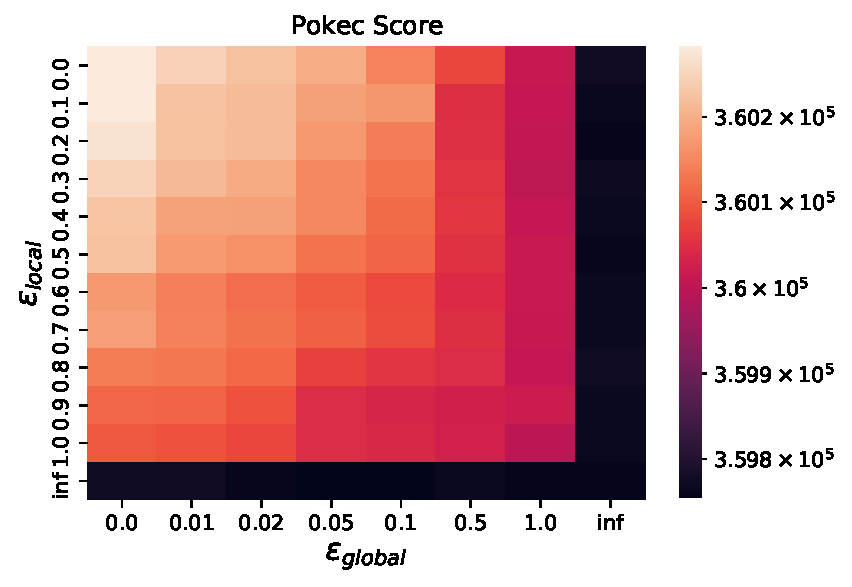
\includegraphics[width=0.33\linewidth]{images/heatmap_Pokec_score.pdf}\\
    \end{center}
    \caption{Effect of $\epsilon$ parameters on \acro's performance.}\label{fig:parameter-smallmultiples} 
\end{figure*}    

Even though, \acro's behavior is not chaotic with respect to changes in parameters. Our method's performance, both in terms of speed and quality of results, depends on parameter selection. Setting $\epsilon_local$ to $0$ means that \acro will always rebuild sketches, which would slowdown the method but it will give the best possible results. On the other hand, setting $\epsilon_local$ to infinity will be very fast, since sketches are build only once without checking vertices blocked. But, quality of the results will suffer.  


\begin{algorithm}
\caption{\sc{\acro}($G,K,J$)}
\label{algo:main}
\algorithmicrequire{$G = (V,E)$: the influence graph
\\\hspace*{6.6ex}{$K$: number of seed vertices
\\\hspace*{6.7ex}$\mathcal{J}$: number of MC simulations}\\}
\algorithmicensure{$S$: a seed set that maximizes influence on $G$
}
\begin{algorithmic}[1]
    \State {$S \leftarrow \{\emptyset\}$}
    \For{$ v\in V$} {\bf in parallel}
        \For{$ j\in J$}
            \State $M[j]_v \leftarrow clz(hash(v) \oplus hash(j))$ 
        \EndFor
    \EndFor
    \State $M \leftarrow simulate(G,M,\emptyset)$
    \State $mask \leftarrow zeros(J)$
    \State $\varsigma \leftarrow 0$
    \For{$k=1\ldots K$}
        \State $s \leftarrow \underset{v\in V}{\mathrm{argmax}} ~estimate(merge(mask,M_v))$
        \State $S \leftarrow S \cup \{s\}$
        \State $e \leftarrow estimate(merge(mask,M_s))$
        % \State $R_S \leftarrow run\_cascade(G,S,J)$
        \State {Compute seed set $S$'s Reachability set $R_{G}(S)$ }
        \State $\sigma_G(S) \leftarrow |R_{G}|/J$
        \State $\delta = \sigma - \varsigma$
        \If{$ (e - \delta) / \delta < \epsilon_l \lor |e-\delta| / \sigma < \epsilon_g$}
            \State $mask \leftarrow merge(mask,M_s)$
        \Else
            \For{$ v\in V$} {\bf in parallel}
                \For{$ j\in J$}
                    \State $M[j]_v \leftarrow clz(hash(v) \oplus hash(j))$ 
                \EndFor
            \EndFor
            \State $M \leftarrow simulate(G,M,R_S)$
            \State $mask \leftarrow zeros(J) $ 
            \State $\varsigma \leftarrow \sigma $ 
        \EndIf
    \EndFor
    \State \Return $S$
\end{algorithmic}
\end{algorithm}

\begin{algorithm}[!ht]
\caption{\sc{Simulate}($G,M,J,R_S$)}
\label{algo:diffusion-step}
\algorithmicrequire{$G = (V,E)$: the influence graph
\\\hspace*{6.6ex}{$M$: Sketch vectors of vertices
\\\hspace*{6.7ex}$\mathcal{J}$: number of MC simulations
\\\hspace*{6.7ex}$R_S$: Reachability set of the seed set
}
\\}
\algorithmicensure{$M$: Updated Sketch vectors
}
\begin{algorithmic}[1]
    \State {$L \leftarrow V$}
    \State {$L' \leftarrow {\emptyset}$}
    \While{$|L|/|V| > \epsilon_c$}
        \For{$u \in \Gamma(L)$} {\bf in parallel} \label{ln:inner_start} %REVERSE THIS
        \For{$e_{u,v} \in A(u) $}
            \For{$j \in (0,J]$}
                \If{$P(u,v)_j < w_{u,v} \land u  \not\in R_S[j]$} \label{ln:early_exit}
                    \State{$M_u[j]\leftarrow max(M_u[j],M_v[j])$}\label{ln:update}         
                \EndIf
            \EndFor
            \If {$M_u$ changed}
                \State $L' \leftarrow L' \cup u $ \label{ln:inner_end}
            \EndIf
        \EndFor
        \EndFor
        \State $L \leftarrow L'$
        \State $L' \leftarrow \{\emptyset\}$
    \EndWhile
    \State \Return $M$
\end{algorithmic}
\end{algorithm}

\subsection{Regularization and Performance considerations}
Traditional two-step, sample-then-diffuse computation model stores data loosely-coupled. Sampled edges are stored together, diffusion related information stored afar. This way, SIMD operation is allowed on consecutively located edges, requiring random memory accesses for the diffusion process. Even if samples or diffusion information stored closely, without fusing random access overhead is still there and much memory is wasted. 

One of the main advantages of fused sampling is allowing similar simulation data and computations together. For processing samples for an edge in algorithm \ref{algo:diffusion-step}~(lines~\ref{ln:inner_start}--\ref{ln:inner_end}).  

 All memory registers from different simulations are stored together for each vertex, this allows the use of vectorized computation hardware. Random number generation, sampling, and merging sketches are all vectorizable operations when coupled together. Vectorization also reduces branching on overall computation; When vectorized, many comparison operations are done without branching. 

We allow a single easy to predict branch after sample edges are generated to exit early without merging the registers. In our experiments, sorting random values $X_r$ significantly increases performance by clustering similar simulations together. Since sorted random values are XOR'ed with the same edge hash values, it is more likely to non-taken edges are sampled together. Up to 20\% performance can be gained by an early exit at line \ref{ln:early_exit} using sorted random values.

\subsection{Implementation Details}
The Compressed Sparse Row~(CSR) graph data the structure used by all the algorithms. 
In CSR, an array, $index$, holds the starting indices of each neighboring vertex, while another vector, $adj$, holds consecutive neighbors of each vertex. 
To enter the neighbors of vertex $i$ we first visit $index[i]$ and $index[i+1]$ 
to find the data's start and end positions, then search from $adj[index[i]]$ to $adj[index[i+1]]$. 
    
\section{Evaluation}\label{sec:evaluation}
We performed the experiments on a server with {\tt Intel Xeon Gold 6140}, running at 2.3 Ghz and 250 GB memory. All of the 18 cores are allowed in the experiments. The Operating System on the server was {\tt Ubuntu 16.04 LTS} with 5.4.0-48 kernel. The algorithms are implemented using {\tt C++20}, and compiled with {\tt GCC 9.2.0} with {\tt "-Ofast"} and {\tt "-march=native"} optimization flags. Multi-thread parallelization was achieved with {\tt OpenMP} pragmas. {\tt AVX2} instructions are utilized by handcrafted code with vector intrinsics.

\begin{table}[!ht]
\caption{Properties of networks used in the experiments}\label{tab:NetProps}
\centering
\scalebox{0.95}{
\begin{tabular}{ll||r|r|r|r}
& & No. of           & No. of    & Avg.  &  Avg.  \\
&Dataset & Vertices          & Edges     &    Weight         &  Degree               \\
\hline
\multirow{6}{*}{\rotatebox[origin=c]{90}{Undirected}}& {\tt Amazon} & 262,113 & 1,234,878 & 1.00 & 4.71 \\
&{\tt DBLP} & 317,081 & 1,049,867 & 1.00 & 3.31 \\
&{\tt NetHEP} & 15,235 & 58,892 & 1.83 & 3.87 \\
&{\tt NetPhy} & 37,151 & 231,508 & 1.28 & 6.23 \\
&{\tt Orkut} & 3,072,441 & 117,185,083 & 1.00 & 38.14 \\
&{\tt Youtube} & 1,134,891 & 2,987,625 & 1.00 & 2.63 \\

\hline
\multirow{6}{*}{\rotatebox[origin=c]{90}{Directed}}&{\tt Epinions} & 75,880 & 508,838 & 1.00 & 6.71 \\
&{\tt LiveJournal} & 4,847,571 & 68,993,773 & 1.00 & 14.23 \\
&{\tt Pokec} & 1,632,803 & 30,622,564 & 1.00 & 18.75 \\
&{\tt Slashdot0811} & 77,360 & 905,468 & 1.00 & 11.70 \\
&{\tt Slashdot0902} & 82,168 & 948,464 & 1.00 & 11.54 \\
&{\tt Twitter} & 81,306 & 2,420,766 & 1.37 & 29.77 
\end{tabular}
}
\end{table}
\subsection{Experiment Settings}

We performed experiments on twelve graphs~(six undirected, six directed) are used in the experiments. For relevancy, datasets that are frequently used for Influence Maximization are selected.

The datasets are {\tt Amazon} co-purchase network~\cite{snapnets}, {\tt DBLP} co-laboration network~\cite{snapnets}, {\tt Epinions} consumer review trust network, {\tt LiveJournal}~\cite{snapnets}, {\tt NetHEP} citation network~\cite{MixGreedy}, {\tt NetPhy} citation network~\cite{MixGreedy}, {\tt Orkut}~\cite{snapnets}, {\tt Pokec} Slovakian poker game site friend network~\cite{snapnets}, {\tt Slashdot} friend-foe networks~(08-11, 09-11)~\cite{snapnets}, {\tt Twitter} list co-occurence network~\cite{snapnets}, and {\tt Youtube} friendship network~\cite{snapnets}. The properties of these datasets are given in Table~\ref{tab:NetProps}. 

The properties of these datasets are given in Table~\ref{tab:NetProps}. 

Three diffusion settings are simulated for a comprehensive experimental evaluation; for each network, we use 
\begin{enumerate}
    \item constant edge weights $w = 0.005$,
    \item constant edge weights $w = 0.01$~(as in~\cite{kempe2003maximizing} and~\cite{MixGreedy}),
    \item constant edge weights $w = 0.1$~(as in~\cite{kempe2003maximizing}),
    % \item weighted cascade edge weights $w_{u,v} = 1/|\Gamma(v)|$.
\end{enumerate}

We selected $w=0.005$ as one of our benchmark settings to challenge ourselves; Due to the nature of the diffusion algorithm, \acro traverses vertices even if they are blocked. Also, for each live vertex \acro generates sample edges for all simulations regardless. Small $w$ values increases overhead operations we mentioned. The other two experiment settings are used to emulate experiments of Kempe et al.~\cite{kempe2003maximizing}


\subsection{Performance Metrics}


In this paper, the algorithms are evaluated on execution time, influence score, and maximum resident memory use. In computing, these three are
often traded off to each other; In the extreme, it is trivial to select random vertices as seed set or compute reachability sets of every possible seed set combination. 

The observed execution times and memory consumption of different algorithms are comparable when the algorithms run on the same computer.
In this paper, the execution time measured is always the wall time reported by the programs. 
All methods we benchmarked leave out the time spend on reading files and pre-processing. To be fair in evaluating our method, we only left out the time to spend on reading files, and respected authors' measurement schemes in other methods. 
In all benchmarks, we allowed methods to fully utilize all available CPU cores, except {\sc Tim+} which is a single-threaded software. Memory use we reported is Resident Set Size(RSS) and measured using GNU Time software.

Although, because the algorithms can use various methods to measure the impact score, the reported influence scores may be deceptive. 
Due to reason, we implemented an oracle with a very simple, sample-than-diffuse algorithm without any optimization mentioned. The random oracle values are generated by the 32-bit Mersenne Twister pseudo-random generator with a state size of 19937 bits {\tt mt19937} from {\tt C++ standard library}. All influence scores in this paper are reported with the independent oracle.


\subsection{Algorithms evaluated in the experiments}

We evaluated our method against three other state-of-the-art influence maximization algorithms, {\sc Tim+}, {\sc Skim}, and {\sc Imm}.

First, Two-phased Influence Maximization({\sc Tim+})~\cite{tim},TIM consists of two phases, Parameter Estimation and Node Selection. The first phase computes a lower-bound
of the maximum expected to spread among all size-k node sets,
and then uses the lower-bound to derive a parameter $\theta$. In the second phase, samples $\theta$ random RR sets from
G, and then derives a size-k node-set $\hat{S}$ that covers a large number of RR sets.

Second, Sketch-based Influence Maximization({\sc Skim})~\cite{cohen2014sketch} constructs bottom-$K^2$ min-hash sketches to estimate the reachability and utilizes multi-thread parallelization in some degree. 

Third, Minutoli et al.'s {\sc Imm}~\cite{minutoli2019fast}. 
{\sc Imm} is a fast algorithm that efficiently produces accurate seed sets. 
The {\sc Imm}  algorithm\cite{tang2015influence} is an approximation method that improves the Reverse Influence Sampling(RIS)\cite{borgs2014maximizing} algorithm By eliminating the need for the threshold to be used.

The influence of all vertices is generalized on a small set of sample graphs that is sampled from reachability sets of few vertices.  Experimentations are done with $\epsilon = 0.5$ as suggested in the original paper, where $\epsilon$ is a user-defined hyper-parameter controlling the approximation boundaries.

Finally, our method \acro employs both Monte-Carlo simulations and count-distinct sketches for estimating reachability set cardinalities. Even-though, \acro is blazing-fast and accurate for limited $K$, we exploit the performance of the method to improve results by rebuilding sketches after removing residual influence networks.

%%%%%%%%%%%%%%%%%%%%%%%%%%%%%%%%%%%%%%%%%%%%%%%%%%%%%%%%%%%%%%%%%%%%%


\begin{table*} %TABLE 5+7
    \caption{\acro execution times~(in secs), memory use~(in GBs), and influence scores on the networks with $K = 50$ seeds using $\tau=18$ threads and constant edge weights $w=0.005$. Influence scores are given relative to \acro{}. }
    \label{tab:timings005}
    \centering
    \scalebox{0.96}{


\begin{tabular}{l|rrrr|rrrr|rrrr}
\toprule
{} & \multicolumn{4}{c|}{Time} & \multicolumn{4}{c|}{Score} & \multicolumn{4}{c}{Memory} \\
Method & {\sc HyperFuser} &    {\sc Tim+} &    {\sc Imm} &  {\sc Skim} & {\sc HyperFuser} &    {\sc Tim+} &     {\sc Imm} &    {\sc Skim} & {\sc HyperFuser} &  {\sc Tim+} &  {\sc Imm} & {\sc Skim} \\
Dataset      &            &         &        &       &            &         &         &         &            &       &      &      \\
\midrule
{\tt Amazon}       &       1.30 &  124.38 &   5.58 & 63.73 &       96.9 &  1.041x &  1.000x &  0.562x &       0.17 & 21.62 & 0.90 & 6.78 \\
{\tt DBLP}         &       1.61 &  177.99 &   5.71 & 28.24 &      106.6 &  1.068x &  1.027x &  1.036x &       0.27 & 31.24 & 0.95 & 3.12 \\
{\tt Epinions}     &       1.11 &   12.16 &   0.50 &  8.29 &      635.3 &  1.026x &  1.001x &  0.939x &       0.06 &  0.78 & 0.07 & 1.04 \\
{\tt LiveJournal}  &      13.25 & 4172.69 & 118.82 & 19.35 &    37174.1 &  1.010x &  0.995x &  0.957x &       3.97 & 27.43 & 2.78 & 2.00 \\
{\tt NetHEP}       &       0.31 &    2.22 &   0.31 &  1.96 &       80.2 &  1.065x &  0.993x &  0.871x &       0.01 &  0.80 & 0.04 & 0.33 \\
{\tt NetPhy}       &       0.39 &    7.40 &   0.40 &  1.00 &      124.5 &  1.042x &  0.999x &  0.777x &       0.03 &  2.01 & 0.08 & 0.16 \\
{\tt Orkut}        &      30.22 &       - & 780.22 & 41.82 &   158842.6 &       - &  0.997x &  1.001x &       5.19 &     - & 7.81 & 1.77 \\
{\tt Pokec}        &      11.05 &  149.34 &   5.04 & 18.40 &     1095.1 &  1.032x &  1.027x &  0.925x &       1.57 & 10.16 & 1.40 & 1.74 \\
{\tt Slashdot0811} &       1.18 &    6.93 &   0.40 &  1.00 &      576.4 &  1.015x &  0.983x &  0.942x &       0.06 &  0.76 & 0.09 & 0.13 \\
{\tt Slashdot0902} &       1.14 &    6.96 &   0.40 &  1.17 &      610.5 &  1.022x &  0.998x &  0.953x &       0.06 &  0.71 & 0.08 & 0.14 \\
{\tt Twitter}      &       1.10 &  171.17 &   5.40 &  1.60 &     3458.7 &  1.006x &  0.990x &  0.942x &       0.09 &  2.02 & 0.12 & 0.15 \\
{\tt Youtube}      &       1.95 &   46.61 &   2.42 & 13.24 &     1820.8 &  1.025x &  1.013x &  1.000x &       0.73 &  3.96 & 0.48 & 1.39 \\
\bottomrule
Geo. Mean wrt.&1.00x&28.19x&1.69x&3.46x&1.00x&1.03x&1.00x&0.90x&1.00x&22.75x&1.65x&3.58x \\ \acro
\end{tabular}

    }
    \end{table*}
    
    \begin{table*} %TABLE 5+7
    \caption{\acro execution times~(in secs), memory use~(in GBs), and influence scores on the networks with $K = 50$ seeds using $\tau=18$ threads and constant edge weights $w=0.01$. Influence scores are given relative to \acro{}. }
    \label{tab:timings01}
    \centering
    \scalebox{0.93}{

% \begin{tabular}{lrrrrrrrrrrrr}
% \toprule
% {} & \multicolumn{4}{l}{Time} & \multicolumn{4}{l}{Score} & \multicolumn{4}{l}{Memory} \\
% Method & HyperFuser &    TIM+ &     IMM &   SKIM & HyperFuser &    TIM+ &     IMM &    SKIM & HyperFuser &  TIM+ &   IMM & SKIM \\
\begin{tabular}{l|rrrr|rrrr|rrrr}
\toprule
{} & \multicolumn{4}{c|}{Time} & \multicolumn{4}{c|}{Score} & \multicolumn{4}{c}{Memory} \\
Method & {\sc HyperFuser} &    {\sc Tim+} &    {\sc Imm} &  {\sc Skim} & {\sc HyperFuser} &    {\sc Tim+} &     {\sc Imm} &    {\sc Skim} & {\sc HyperFuser} &  {\sc Tim+} &  {\sc Imm} & {\sc Skim} \\

Dataset      &            &         &         &        &            &         &         &         &            &       &       &      \\
\midrule
{\tt Amazon }       &       0.96 &  107.94 &    3.28 &  59.32 &      152.7 &  1.037x &  1.024x &  0.390x &       0.17 & 18.11 &  0.55 & 6.40 \\
{\tt DBLP }         &       0.73 &   73.37 &    2.85 &  18.71 &      233.5 &  1.043x &  1.005x &  0.997x &       0.27 & 11.92 &  0.52 & 2.05 \\
{\tt Epinions }     &       0.82 &  112.08 &    3.78 &   5.07 &     2480.1 &  1.006x &  0.983x &  0.984x &       0.06 &  1.95 &  0.10 & 0.68 \\
{\tt LiveJournal }  &      16.72 &       - &  386.37 &  16.23 &   155375.8 &       - &  0.996x &  0.993x &       3.97 &     - &  6.64 & 1.45 \\
{\tt NetHEP }       &       0.26 &    1.84 &    0.23 &   1.89 &      129.1 &  1.036x &  0.997x &  0.826x &       0.01 &  0.60 &  0.03 & 0.31 \\
{\tt NetPhy }       &       0.24 &    3.33 &    0.23 &   0.86 &      320.5 &  1.010x &  0.985x &  0.732x &       0.03 &  0.67 &  0.05 & 0.12 \\
{\tt Orkut }        &      42.37 &       - & 1870.35 & 114.82 &   650157.1 &       - &  1.000x &  1.000x &       5.19 &     - & 20.13 & 3.43 \\
{\tt Pokec }        &      11.65 & 4148.03 &   88.89 &   7.25 &    44685.8 &  1.004x &  0.996x &  0.988x &       1.57 & 39.98 &  2.09 & 0.78 \\
{\tt Slashdot0811 } &       0.84 &  102.96 &    3.70 &   0.87 &     2882.1 &  1.003x &  0.984x &  0.976x &       0.06 &  2.01 &  0.10 & 0.08 \\
{\tt Slashdot0902 } &       0.90 &  129.31 &    4.19 &   0.88 &     3061.5 &  1.008x &  0.992x &  0.980x &       0.06 &  2.42 &  0.11 & 0.08 \\
{\tt Twitter }      &       0.90 &  390.36 &   10.96 &   1.22 &     9628.6 &  1.004x &  0.992x &  0.978x &       0.09 &  4.91 &  0.23 & 0.09 \\
{\tt Youtube }      &       2.18 &  534.41 &   14.86 &  16.97 &     9042.7 &  1.009x &  0.994x &  1.006x &       0.73 &  7.10 &  0.48 & 1.73 \\
\bottomrule
Geo. Mean wrt.&1.00x&100.14x&5.45x&3.58x&1.00x&1.02x&1.00x&0.88x&1.00x&36.26x&1.91x&2.82x \\ \acro
\end{tabular}



    }
    \end{table*}
    \begin{table*} %TABLE 5+7
    \caption{\acro execution times~(in secs), memory use~(in GBs), and influence scores on the networks with $K = 50$ seeds using $\tau=18$ threads and constant edge weights $w=0.1$. Influence scores are given relative to \acro{}. }
    \label{tab:timings1}
    \centering
    \scalebox{0.90}{

\begin{tabular}{l|rrrr|rrrr|rrrr}
\toprule
{} & \multicolumn{4}{c|}{Time} & \multicolumn{4}{c|}{Score} & \multicolumn{4}{c}{Memory} \\
Method & {\sc HyperFuser} &    {\sc Tim+} &    {\sc Imm} &  {\sc Skim} & {\sc HyperFuser} &    {\sc Tim+} &     {\sc Imm} &    {\sc Skim} & {\sc HyperFuser} &  {\sc Tim+} &  {\sc Imm} & {\sc Skim} \\
Dataset      &            &         &         &        &            &         &         &         &            &        &       &      \\
\midrule
{\tt Amazon}       &       0.69 &  133.22 &    1.98 &  23.62 &    11797.0 &  1.006x &  0.990x &  0.815x &       0.17 &   5.49 &  0.23 & 2.59 \\
{\tt DBLP }         &       0.54 & 1368.83 &   14.54 &   6.30 &    48549.9 &  1.001x &  0.995x &  1.001x &       0.27 &  35.19 &  1.06 & 0.65 \\
{\tt Epinions }     &       0.26 &  439.33 &    5.46 &   9.42 &    18409.9 &  1.000x &  0.998x &  0.997x &       0.06 &  12.17 &  0.39 & 1.18 \\
{\tt LiveJournal }  &      10.10 &       - & 1071.30 &  65.73 &  2134726.0 &       - &  1.000x &  1.000x &       3.97 &      - & 65.49 & 1.40 \\
{\tt NetHEP }       &       0.10 &   14.18 &    0.33 &   0.61 &     2461.7 &  1.002x &  0.975x &  0.899x &       0.01 &   1.02 &  0.04 & 0.10 \\
{\tt NetPhy }       &       0.16 &  107.52 &    1.53 &   0.34 &     8339.5 &  1.007x &  0.994x &  0.975x &       0.03 &   3.84 &  0.13 & 0.03 \\
{\tt Orkut }        &      16.55 &       - & 1964.83 & 446.92 &  2692366.5 &       - &  1.000x &  1.000x &       5.19 &      - & 71.94 & 9.68 \\
{\tt Pokec }        &       4.90 &       - &  514.79 &  31.80 &  1034859.8 &       - &  1.000x &  1.000x &       1.57 &      - & 26.46 & 0.98 \\
{\tt Slashdot0811 } &       0.21 &  677.49 &    7.34 &   2.44 &    25871.8 &  1.000x &  1.000x &  0.999x &       0.06 &  19.10 &  0.59 & 0.25 \\
{\tt Slashdot0902 } &       0.23 &  695.12 &    7.99 &   2.35 &    27519.5 &  1.000x &  1.000x &  0.999x &       0.06 &  18.45 &  0.66 & 0.24 \\
{\tt Twitter }      &       0.33 & 1897.50 &   16.09 &   1.62 &    55327.3 &  1.000x &  0.998x &  0.998x &       0.09 &  34.56 &  1.04 & 0.05 \\
{\tt Youtube }      &       1.12 & 7158.56 &   60.59 &  30.57 &   171392.9 &  1.000x &  0.999x &  1.001x &       0.73 & 139.12 &  4.19 & 2.88 \\
\bottomrule
Geo. Mean wrt.&1.00x&1449.41x&27.87x&11.06x&1.00x&1.00x&1.00x&0.97x&1.00x&163.77x&7.14x&2.63x \\ \acro
\end{tabular}


    }
    \end{table*}
    
 \begin{figure}[!h] 
     \centering
     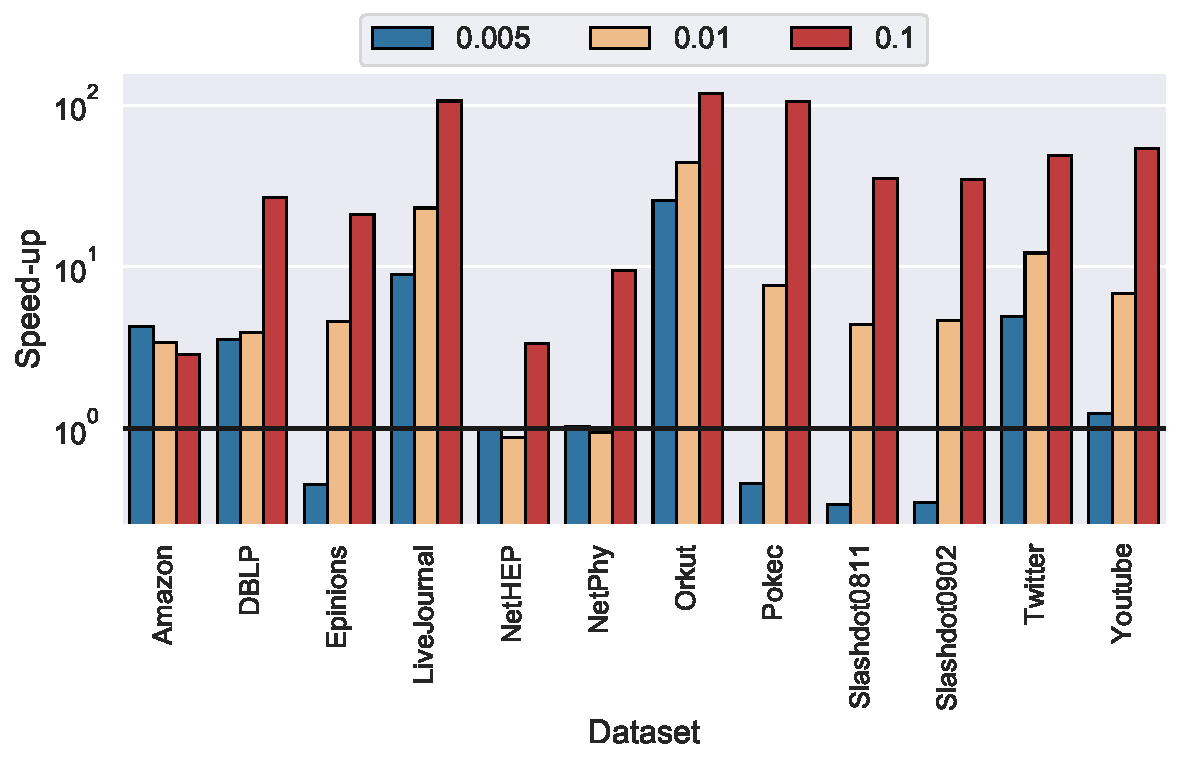
\includegraphics[width=1\linewidth]{images/speedup-imm}
   \centering \caption{Speed-up obtained by \acro{} over {\sc Imm}($\epsilon\myeq 0.5$) using $\tau=18$ threads.
     \label{fig:vs-imm}} 
 \end{figure}

 \begin{figure}[!h] 
     \centering
     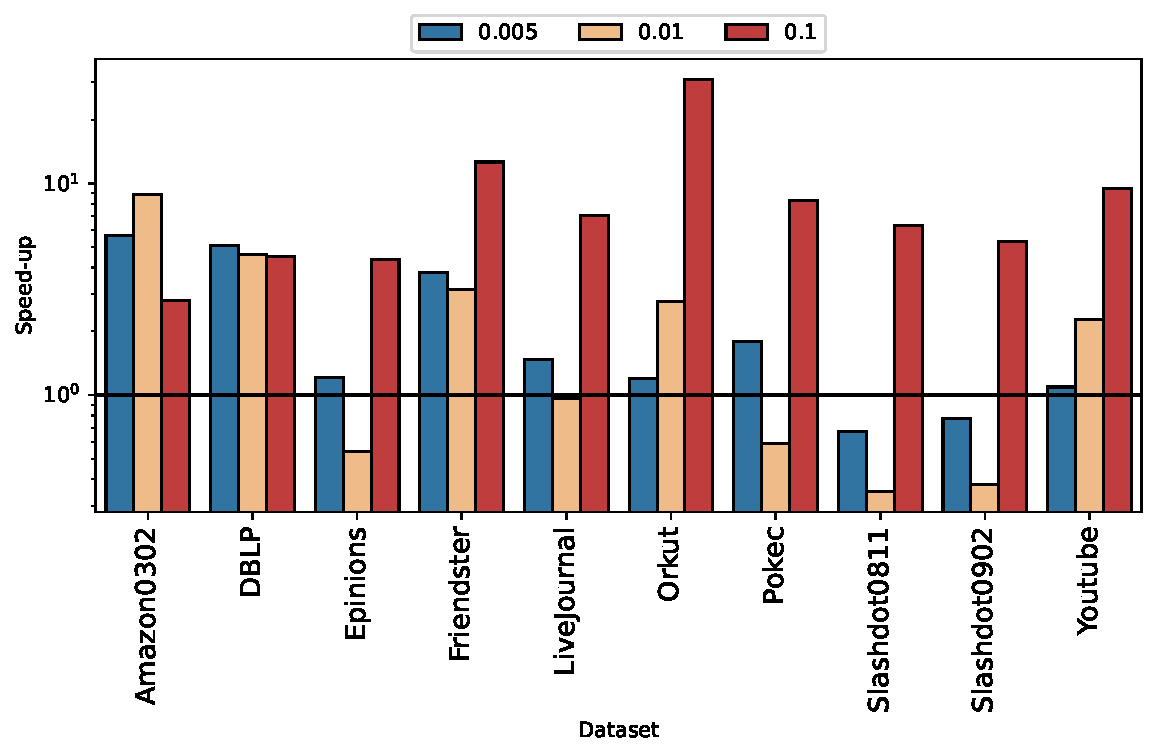
\includegraphics[width=1\linewidth]{images/speedup-skim}
   \centering \caption{Speed-up obtained by \acro{}($J=256$) over {\sc Skim}($r\myeq 64,l\myeq 64$) using $\tau=18$ threads.
     \label{fig:vs-skim}} 
 \end{figure}


\subsection{Scalability with multi-threaded parallelism}

\begin{figure*}[!ht] 
    \centering
    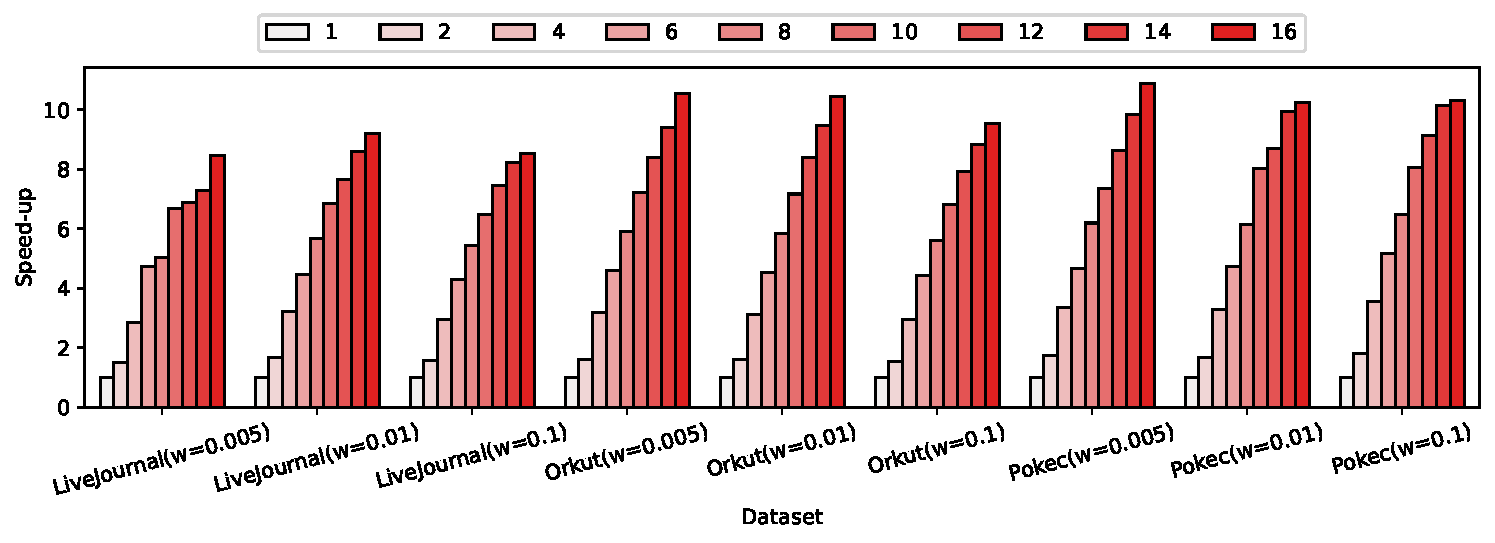
\includegraphics[width=\linewidth]{images/threads.pdf}
   \centering \caption{\acro scaling with multiple threads on some of largest datasets in the benchmarks.
     \label{fig:scaling}} 
\end{figure*}


In our implementation, the parallel processing of live vertices  (as source) is necessary to reduce the number of visited edges. However, since a (target) vertex can be being processed at the same time, the update operation at line~\ref {ln:update} of this {\em pull-based} approach can be seen as a potential source of race conditions. But, since iterations are performed until convergence, the results are sound within our assumptions. On the other hand, the performance may suffer due to false sharing.
Figure~\ref{fig:scaling} shows the speedup values obtained via {\tt OpenMP} parallelization.

Even though {\em pull-based} diffusion approach we employed in this work gives us superior performance in most of the benchmarks, it is possible to implement \acro using other approaches; E.g. {\em queue-based} approach is similarly feasible and may improve performance by only processing live vertices. The pull-based diffusion method is chosen due to its simplicity and scalability to a large number of threads/compute units. 

\subsection{Comparing \acro with State-of-art}
All algorithms mentioned in this paper, estimates influence maximizing seed sets, that are good enough but not optimal. For that reason, we compare both the performance and quality of the results. In addition to this trade-off, the parameters of the experimented methods are hard to compare directly. It is infeasible to find exactly the corresponding parameter between any two methods in this setting. For that reason, we have used parameters that authors of the methods used in their papers.
We performed experiments using following parameters; {\sc Tim+} ($\epsilon=0.3$), {\sc Imm} ($\epsilon=0.5$), {\sc Skim} ($l=64,k=64$). 

One of the drawbacks of \acro is that we do not have direct control over the approximation factor whereas other methods we compare against some form of an approximation control parameter. \acro can only control approximation quality indirectly by tuning the number of Monte-Carlo simulations $J$, and to some degree with estimation/convergence thresholds. 
For \acro, we used $J=256$ registers which is comparable in terms of quality of other methods. And, for performance we used global estimation error threshold $\epsilon_{global}=0.01$, local estimation error threshold $\epsilon=0.3$, and set non-converged vertices ratio as $\epsilon_{conv}=0.02$. 


For small $w=0.005$ and small graphs such as NetHep, NetPhy, or Amazon; we can see {\sc Tim+}  has ($4\sim 6\%$) better results, whereas {\sc Skim}  has much ($- 13\sim 44\%$) worse results than \acro in terms of quality. While \acro having a hard time to catch edges in samples; \acro has a chance of capturing an edge is $1-(1-0.005)^{256}=0.72$, {\sc Tim+} won't suffer from the situation but {\sc Skim}  suffer much worse capturing vertices in sketches. On the performance side, \acro is superior to other methods, Amazon dataset only takes 1.3 seconds including Monte-Carlo influence oracle computations. {\sc Skim} and {\sc Imm} take 63.73 and 124.38 seconds. For 4\% quality improvement, {\sc Imm} is $\sim$100 slower than \acro. For small improvements in quality, we can always double the number of registers/simulations $J=256$ to $512$, which would approximately double the wall time. For the same $w=0.005$ and larger graphs such as {\tt LiveJournal} and {\tt Orkut}, the quality gap narrows {\sc Skim}  only $5\%$ behind, and {\sc Tim+} is marginally better. 
The performance gap also narrows between \acro and {\sc Skim}, \acro only $30\%$ faster in small $w$. In the same setting, {\sc Tim+}  takes 1.5 hours for {\tt LiveJournal}, could not finish {\tt Orkut}; crashing after consuming all memory available. 
For $w=0.1$, \acro is much faster than all other methods and still providing high-quality results. While all methods are struggling with problem size, \acro is converging results much faster, even faster than previous experiment settings. Also, memory consumption stays the same for all experimental settings, much smaller than other methods.

\section{Related Work}\label{sec:relatedwork}

Although they can be inferior in terms of influence score, recent IM algorithms are shown to be quite fast compared to conventional simulation-based approaches such as {\sc MixGreedy}. 
% However, in this work, we show that \acro{}, which is a conventional algorithm, can be orders of magnitude faster than {\sc MixGreedy} while keeping the quality of the seed vertices the same. 
Techniques such as using GPUs, sketches for finding set intersections, reverse sampling to estimate influence from a small subset of vertices, and estimating the necessary number of simulations/samples required for each step greatly reduces asymptotic boundaries of execution time~\cite{leskovec2009community, borgs2014maximizing, minutoli2019fast, cohen2014sketch, IPA, IMGPU, curipples}. 

\acro borrows much from {\sc InFuseR}~\cite{infuser}, including hash-based fused sampling and vertex parallel diffusion algorithm. {\sc InFuseR} computes influence by memoizing connected-components for all vertices and only works on {\em undirected} datasets. Also, employs CELF optimizations to reduce candidate seed set cardinality computations. Whereas, \acro can process both directed and undirected graphs, and uses sampled Flajolet–Martin sketches to both estimate cardinalities and choose candidates. 

Sketch-based influence maximization improves theoretical efficiency against simulation-based methods. The sketch-based approach pre-computes sketches for evaluating the influence spread instead of running simulations repetitively. One of the interesting methods for sketch-based influence maximization is {\sc Skim} ~\cite{cohen2014sketch} by Cohen~et~al. It constructs bottom-$K^2$ min-hash sketches to estimate the reachability and utilizes multi-core, multi-CPU parallelization. 

Independent Path Algorithm~(IPA)~\cite{IPA} by Kim~et~al runs a proxy model and prunes paths with probabilities less than a given threshold. IPA uses {\tt OpenMP} to work on independent paths in parallel. The approach only keeps a dense but small part of the network and scalable on only sparse networks. Liu~et~al. proposed IMGPU~\cite{IMGPU}, an IM  estimation method by utilizing a bottom-up traversal algorithm. It performs a single Monte-Carlo simulation on many GPU threads to find the reachability of the seed set. It is $5.1\times$ faster than {\sc MixGreedy} on a CPU. The GPU implementation is up to $60\times$ faster with an average speedup of  $24.8\times$.

Borgs~et~al.~\cite{borgs2014maximizing} proposed Reverse Influence Sampling~(RIS) which samples a fraction of all random reverse reachable sets. Then it computes a set of $K$ seeds that covers the maximum number of those. The number of samples is calculated concerning the number of visited vertices. The algorithm has an approximation guarantee of $(1-1/e-\epsilon)$. Minutoli et al.~improved RIS and proposed {\sc Imm} that works on multi-threaded and distributed architectures~\cite{minutoli2019fast}. 
Recently, the authors extended the algorithm to work on GPUs~\cite{curipples}.   

Two-phased Influence Maximization({\sc Tim+} )\cite{tim} borrows ideas from RIS but overcomes its limitations with a novel algorithm design. The first phase computes a lower-bound of the maximum expected to spread among all size-k node sets, and then uses the lower-bound to derive a parameter $\theta$. In the second phase, samples $\theta$ random RR sets from G, and then derives a size-k node-set $\hat{S}$ that covers a large number of RR sets.

Cohen\cite{cohen2015all} presented the Historic Inverse Probability (HIP) estimators. When applied to the All Distance Sketches, HIP outperforms in estimation quality of the HyperLogLog sketches\cite{flajolet2007hyperloglog} for approximate distinct counting on data streams. In this work, we preferred Flajolet-Martin\cite{flajolet1985probabilistic} sketches for simplicity and performance. In future work, other estimators such as HIP can improve to improve \acro.

Kumar and Calders\cite{kumar2017information} proposed Time Constrained Information
Cascade Model and an influence maximization algorithm that works on the model using versioned HyperLogLog sketches. The algorithm performs the influence reachability sets for all vertices in an interaction graph performing a single pass over the data. Sketches build for each time window to estimate active edges where as \acro builds sketches for each vertex to estimate the cumulative influence of the latent seed set. \acro also utilizes fused sampling and error adaptive rebuilding of sketches.

\section{Conclusion and Future Work}\label{sec:conclusion}

In conclusion, we propose a sketch-based Influence Maximization algorithm that employs fused sampling and error-adaptive rebuilding. We provide a fast implementation of the algorithm that utilizes multi-threading to exploit multiple CPU cores. In addition, we present a performance comparison with state-of-the-art IM algorithms on real-world datasets. 
With the proposed method, \acro{} can achieve $\maxspeedupSKIM\times$ speed-up against {\sc Skim} and $\maxspeedupIMM\times$ speed-up against {\sc Imm} while producing high quality results. 

In the future, we would like to extend our work to a distributed GPGPU setting to process graphs with billions of vertices and edges. The main issue with \acro on such computation scheme is the broadcast of sketch registers; when vertices are partitioned to different computation units, resulting sketch updates should be communicated to all partitions. To overcome the issue, graph pre-processing and speculative diffusion strategies can reduce communication bottlenecks. 

%%%%%%%%%%%%%%%%%%%%%%%%%%%%%%%%%%%%%%%%%%


\ifCLASSOPTIONcaptionsoff
  \newpage
\fi


\bibliographystyle{IEEEtran}
\bibliography{refs}
\begin{IEEEbiography}[{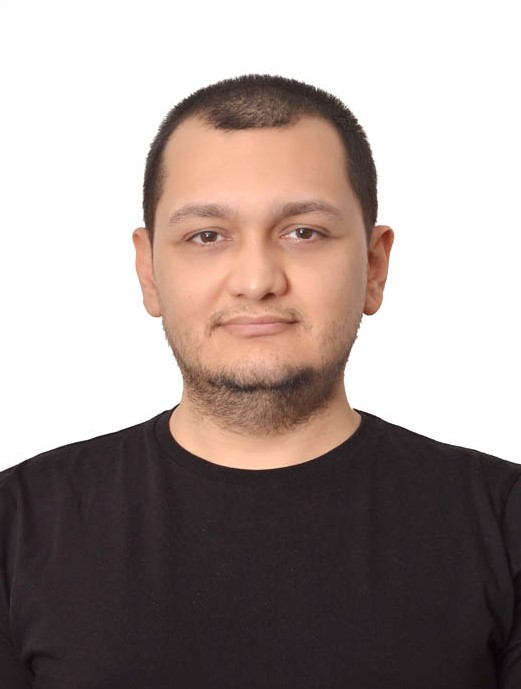
\includegraphics[width=1in,height=1.25in,clip,keepaspectratio]{./images/gokhan.png}}]{G\"{o}khan~G\"{o}kt\"{u}rk} is a PhD candidate at the Faculty of Engineering and Natural Sciences in Sabancı University. He has received his BS and MS degrees from Sabancı University as well. He is interested in High Performance Computing, Parallel Programming, and Graph Processing.
\end{IEEEbiography}
\begin{IEEEbiography}[{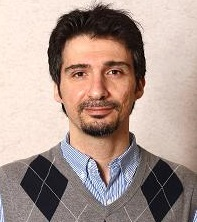
\includegraphics[width=1in,height=1.25in,clip,keepaspectratio]{./images/kamer.jpg}}]{Kamer Kaya} is an Assistant Professor at the Faculty of Engineering and Natural Sciences at Sabancı University. He got his PhD from Dept. Computer Science and Engineering from Bilkent University. He worked at CERFACS, France, as a post-graduate researcher in the Parallel Algorithms Project. He then joined the Ohio State University in September 2011 as a postdoctoral researcher, and in December 2013, he became a Research Assistant Professor in the Dept. of Biomedical Informatics.
His current research interests include Parallel Programming, High-Performance Computing, and Cryptography. 
    \end{IEEEbiography}

\end{document}


